\documentclass[10.5pt, a4paper, twoside, openright]{report}

% -- English --
%\usepackage[english]{babel}
% -- French  --
\usepackage[russian, francais]{babel}
\usepackage[T2A, T1]{fontenc}
\usepackage[utf8]{inputenc}
\usepackage[a4paper, left=2cm, right=2cm, top=2.5cm, bottom=2cm, headheight=40pt]{geometry}
\usepackage{graphicx}

% -- Layout --
\usepackage{algorithm}
\usepackage{algcompatible}
\usepackage{algorithmicx}
\usepackage{algpseudocode}
\usepackage{bytefield}
\usepackage[table]{xcolor}
\usepackage{listings}
\lstset{extendedchars=true, inputencoding=latin1,
  backgroundcolor=\color{black!5}, basicstyle=\footnotesize,}
\usepackage{tikz}
\usetikzlibrary{shapes}
\usetikzlibrary{patterns}
\usepackage{hyperref}
\usepackage{emptypage}
\usepackage{fancyhdr}
\pagestyle{fancy}
\renewcommand{\headrulewidth}{1pt}
\renewcommand{\chaptermark}[1]{\markboth{#1}{}}
\fancyhead[C]{\leftmark}
\fancyhead[RE,LO]{}
\fancyhead[RO,LE]{
\includegraphics[scale=0.016]{UB.jpg}}
\newcommand{\HRule}{\rule{\linewidth}{0.5mm}}
\raggedbottom{}

\title{Analyse de malware statique et dynamique : Les outils et quelques cas pratiques}
\author{Erwan Grelet \& Amélie Guémon}

\begin{document}

% -- Title Page --
\begin{titlepage}
  \begin{sffamily}
  \begin{center}

    Univesity of Bordeaux\\College of Science \& Technology\\
           351 Cours de la Liberation\\33400 Talence\\[1em]
            \textbf{\underline{- Projet M2 -}}\\[1.5cm]

    
\includegraphics[scale=0.11]{UB.jpg}
    \\[3cm]

    \HRule\\[0.3cm]
    { \huge \bfseries Analyse de malware statique et dynamique : \\Les outils et quelques cas pratiques\\[0.5cm] }
    \HRule\\
    \begin{flushright}
      \bfseries {Erwan GRELET \& Amélie GUÉMON\\[1em]Master 2 CSI --- Cryptology \& Computer Security}\\[6cm]
    \end{flushright}

    \today

  \end{center}
  \end{sffamily}
\end{titlepage}

\tableofcontents

% -- New Part --

\chapter*{Introduction}

Non sans étonnement, l'année 2016 aura été l'année du boom des ransomwares.
Avec 1,3 millions de nouveaux ransomwares détectés lors du second trimestre par
les équipes de McAfee et plus de 90\% des emails de phishing présentant des
ransomwares\footnote{\url{https://phishme.com/phishing-ransomware-threats-soared-q1-2016/}}
, la menace n'est pas à prendre à la légère.
En début d'année, un hôpital californien avait été la cible d'un ransomware,
chiffrant les données médicales de près de milliers de patients(TODO).
L'hôpital aura finalement versé 17.000\$ en bitcoins
(40 bitcoins à cette époque) afin de continuer à
pouvoir soigner ses clients (les auteurs ont accepté un prix plus faible,
la rançon originelle était de 3.4 millions de dollars)\footnote{\url
  {http://khn.org/morning-breakout/california-hospital-held-hostage-by-hackers-pays-17000-ransom-to-unlock-records/}}.
La monétisation d'informations volées ou verrouillées peut rapporter gros aux
auteurs de ces attaques.\\

Mais les ransomwares ne sont pas les seuls malwares à surveiller: ils ne
représentent qu'une partie d'une menace bien plus importante. Des spywares
(rootkits, trojans, keyloggeurs) aux downloaders et botnets,
les menaces sont variées et les cibles de plus en plus diversifiées,
avec l'essor des objets connectés (IoT) et des mobiles. Ces derniers ne
sont pas toujours sécurisés et en font des cibles de choix.\\
Il est donc important de constamment étudier ces nouvelles menaces, afin de
pouvoir protéger les systèmes d'informations et les données qu'ils contiennent.
L'analyse de malware sert typiquement trois causes:
l'obtention d'informations nécessaires à la réponse
à une intrusion, l'extraction d'indicateurs de compromission ou simplement
à la compréhension et la découverte des dernières techniques utilisées
par les fabricants de malwares.\\

Dans ce papier seront donc présentées, en première partie, les techniques
d'analyses de malware, puis deux études de cas pratiques: le botnet Ganiw et
le ransomware SageCrypt.


\chapter{Techniques d'analyses de malwares}

Topo : Introduction analyse statique / dynamique\\

Lors d'une analyse de malware, on a, en général, uniquement accès à l'exécutable quiconstitue le malware. Pour comprendre ce qu'il fait, on doit alors recourir à l'utilisationde nombreux outils et astuces.\\
Il y a deux approches à l'analyse de malwares : statique et dynamique.\\
L'analyse statique consiste à examiner le malware sans l'exécuter, tandis que l'analysedynamique se fait pendant l'exécution du malware. Ces deux approches sont en fait complémentaires et permettent d'obtenir une vision d'ensemble sur le comportement du malware.

\section{Analyse statique}

\subsection{Sacnner anti-virus}

\subsection{Hash du sample et comparaison aux bases de données}

\subsection{Examen de l'exécutable (PE/ELF)}

\begin{itemize}
\item {Symboles}
\item {Fonctions importées / exportées}
\end{itemize}

\subsection{Recherche de chaînes de caractères}

Outils: strings

\subsection{Identification de packing ou d'obfuscation}

\subsection{Analyse du code assembleur}

Outils: Radare2 / IDA Pro

\section{Analyse dynamique}

\subsection{Machine virtuelle (VirtualBox / VMWare}

\begin{itemize}
\item {Mise en réseau}
\item {Snapshots}
\end{itemize}

\subsection{Tracing (strace / ProcMoon)}

\subsection{Listing des processus (ps / ProcessExplorer)}

\subsection{Simulation de réseaux (inetsim)}

\subsection{Analyse de traffic (tcpdump / wireshark)}

\subsection{Debugging (gdb / x64dgb)}

TODO: Notes sur l'automatisation des parties basiques ? (Cuckoo, Limon) <-- Pour !


\chapter{Ganiw}

\section{Introduction}

Le \textit{sample} porté à l'étude porte le doux nom de \textbf{Ganiw} mais est
aussi connu sous les nom de \textbf{BillGates} ou de combinaisons comme
\textbf{LINUX.BACKDOOR.GATES}.\\
Celui-ci semble avoir été étudié pour la première fois en Février 2014
dans un post de \textit{ValdikSS} sur le site \textit{\foreignlanguage{russian}{Хабрахабр}} : \textit{\href{https://habrahabr.ru/post/213973/}
{Studying the BillGates Linux Botnet}}\footnotemark,
mais continue tout de même à être étudié et à être actif.\\

Le malware Ganiw a été réalisé en C++ et pensé de manière à
être modulaire et portable.
Ce malware visait, à l'origine, uniquement les systèmes Linux,
mais a été porté plus tard sur les systèmes Windows\footnotemark.\\
Le choix des systèmes Linux n'est pas anodin, puisque le développement
toujours plus important des objets connectés dans l'"Internet of Things" (IoT).
En effet, une grande partie des systèmes embarqués prenant part à l'IoT fonctionnent
sur des distributions de GNU/Linux (voir OpenWrt\footnotemark ou le projet Yocto\footnotemark).
De plus, ces objets connectés sont, de manière générale, peu ou mal protégés
(absence de firewall, mots de passe faibles,\ldots) et non surveillés ou peu maintenus.
Ce sont donc des cibles de choix pour la création de \textit{botnets},
comme tente de le faire le malware \textbf{Ganiw}, pour mener des attaques
de types DDOS\footnotemark par exemple.\\

\footnotetext{Traduit depuis le russe}
\footnotetext{\url{https://thisissecurity.net/2015/09/30/when-elf-billgates-met-windows/}}
\footnotetext{Distributed Denial-Of-Service}
\footnotetext{\url{https://openwrt.org/}}
\footnotetext{\url{https://www.yoctoproject.org/}}

\subsection{Les outils}

Les principaux outils utilisés pour réaliser cette analyse ont été
le logiciel de virtualisation \href{https://www.virtualbox.org/}{\textit{VirtualBox}},
le debugger GNU \href{https://www.sourceware.org/gdb/}{\textit{GDB}},
l'utilitaire \href{https://github.com/strace/strace}{\textit{strace}},
l'analyseur de paquets \href{https://www.wireshark.org/}{\textit{Wireshark}},
le désassembleur \href{https://github.com/radare/radare2}{\textit{Radare2}} et
et le simulateur de services internet \href{http://www.inetsim.org/}{\textit{INetSim}}
qui sont des logiciels libres.\\

\section{Analyse}

Avant toute chose, voilà, ci-dessous, le SHA-256 du sample analysé :
\begin{lstlisting}
94f5fd896a526427a5ef1de37725e6eae3a06af3da098547f0adcfdd34fbfd2a
\end{lstlisting}

\subsection{Analyse basique}

Pour commencer, il est bon d'utiliser l'utilitaire $file$ pour en apprendre un
peu plus sur l'exécutable :
\begin{lstlisting}
ganiw:  ELF 32-bit LSB executable, Intel 80386, version 1 (SYSV), statically linked,
        for GNU/Linux 2.2.5, not stripped
\end{lstlisting}
C'est donc un exécutable au format ELF (Executable and Linkable Format) 32-bit pour Linux.\\
Il est intéressant de remarquer que l'exécutable est lié statiquement et surtout
qu'il n'a pas été strip (ce qui va nous permettre d'obtenir des informations
utiles telles que les noms de fonctions, méthodes ou variables potentiellement
utilisées par le programme et donc nous permettre de comprendre plus facilement
comment fonctionne le malware).\\

Un petit coup de \textit{strings} nous permet de trouver quelques indices sur
ce qui se passe lors de l'exécution du binaire, par exemple :
\begin{lstlisting}
$> strings ganiw | less 
[...]
/proc/meminfo
MemTotal:         %d kB
/proc/stat
cpu %llu %llu %llu %llu
/proc/net/dev
%7s %llu %lu %lu %lu %lu %lu %lu %lu %llu %lu %lu %lu %lu %lu %lu %lu
/proc/cpuinfo
processor
/proc/net/arp
%16s 0x%d 0x%d %20s %s
%2x:%2x:%2x:%2x:%2x:%2x
/proc/net/route
%5s %8x %8x %s
cpu MHz
cpu MHz         : %d.%d
vector::_M_insert_aux
%5s %s
/bin/netstat
/bin/lsof
/bin/ps
/bin/ss
/usr/bin/netstat
/usr/bin/lsof
/usr/bin/ps
/usr/bin/ss
/usr/sbin/netstat
/usr/sbin/lsof
/usr/sbin/ps
/usr/sbin/ss
GLIBCXX_FORCE_NEW
update_temporary
mkdir -p %s
cp -f %s %s
/tmp/notify.file
/usr/bin/
.lock
[...]
\end{lstlisting}

L'outil \textit{strings} renvoit un grand nombre de chaînes de caractères,
dont certaines intéressantes. Il y a peu de chance que l'exécutable soit
packé ou compressé étant donné le nombre élevé de chaînes claires présentes.\\

L'utilisation de \textit{nm} permet en revanche de voir clairement les symboles présents
dans le binaire. Puisque le malware a été realisé en C++, il est préférable
d'utiliser l'option \textit{-C} de \textit{nm} pour pouvoir lire facilement
le nom des méthodes.\\
Voici, par exemple, ce qu'il est possible de trouver en utilisant \textit{nm} :
\begin{lstlisting}
$> nm -C ganiw | grep Main
080623f2 T MainBeikong()
08061c48 T MainMonitor()
080620ac T MainProcess()
08061d3c T MainSystool(int, char**)
08062304 T MainBackdoor()
08089398 T CThreadTns::ProcessMain()
08083ffe T CThreadDoFun::ProcessMain()
080883fc T CThreadShell::ProcessMain()
08089a3e T CThreadUpdate::ProcessMain()
0807fb5c T CThreadAtkCtrl::ProcessMain()
080865b4 T CThreadHttpGet::ProcessMain()
08087552 T CThreadLoopCmd::ProcessMain()
08087ac0 T CThreadRecycle::ProcessMain()
08087966 T CThreadMonGates::ProcessMain()
08086f2c T CThreadKillChaos::ProcessMain()
08088740 T CThreadTaskGates::ProcessMain()
08083aae T CThreadConnection::ProcessMain()
080848d8 T CThreadFakeDetect::ProcessMain()
08083870 T CThreadClientStatus::ProcessMain()
08083e22 T CThreadFXConnection::ProcessMain()
08088628 T CThreadShellRecycle::ProcessMain()
080808a6 T CThreadKernelAtkExcutor::ProcessMain()
08080db8 T CThreadNormalAtkExcutor::ProcessMain()
08066a8e T CManager::MainProcess()
08066788 T CManager::ZXMainProcess()
08100900 r MainSystool(int, char**)::C.1203
081008c0 r MainSystool(int, char**)::C.1206
\end{lstlisting}
\ \\
Quelques noms intéressants apparaissent, il ne reste plus qu'à aller jeter un
oeil de plus près.\\

Une analyse plus poussée est nécessaire pour avoir une idée concrète de ce que
fait le malware étudié. Pour l'instant, impossible de savoir quels sont les
liens entre les différentes fonctions et méthodes repérées précédemment.
L'analyse continue donc avec Radare2, pour désassembler
le binaire, VirtualBox, GDB et strace pour obtenir des valeurs à des endroits
clés ou la liste des appels systèmes utilisés pendant l'exécution du malware.\\

Afin de faciliter la compréhension des relations qu'entretiennent les
différents modules entre eux, une figure récapitulative est présentée ci-dessous :\\
\begin{figure}[!h]

  \centering
  \begin{tikzpicture}

  \node[draw, minimum width=2cm, text width=2cm, text centered]
  (Be) at (0,0) {Beikong\\BillGates};
  \node[draw, minimum width=2cm, text width=2cm, text centered]
  (Ba) at (5,0) {Backdoor\\Getty};
  \node[draw, minimum width=2cm, text width=2cm, text centered]
  (Mo) at (2,-2.5) {Monitor\\.sshd};
  \node[draw, text centered, shape=diamond]
  (Ta) at (9.5,1.7) {Target};
  \node[draw, minimum width=2cm, text width=2cm, text centered]
  (Us) at (9,-3) {User};
  \node[draw, minimum width=2cm, text width=2cm, text centered]
  (Sy) at (9,-4) {Systool};
  \node[draw, minimum width=2cm, text width=2cm, text centered]
  (OS) at (9,-5.5) {Original\\Systool};
  \node[draw, cloud, cloud puffs=11, minimum height=.5cm,
    minimum width=1.5cm] (CC1) at (0,5) {\shortstack{C\&C}};
  \node (IP) at (-1,6.1) {\shortstack{115.28.206.48:25000}};
  \node[draw, cloud, cloud puffs=11, minimum height=.5cm,
    minimum width=1.5cm] (CC2) at (4.8,5) {\shortstack{C\&C}};
  \node (IP) at (4.5,6.1) {\shortstack{www.i0cc.com}};
  \node[draw, cloud, cloud puffs=11, minimum height=1cm,
    minimum width=1cm] (US) at (2.5,3) {\shortstack{\scriptsize Update\\\scriptsize Server}};

  \draw[-] plot [smooth, tension=0.5] coordinates {(10,-1.8) (7.75,-2.3) (7.75,-6.2) (10,-6.8)};
  \node (Ca) at (9,-7.2) {\shortstack{Cach\'e à\\l'utilisateur}};
  \draw[->, >=latex, thick, color=black!60!green] (Ba.-5) to[bend left]
  node[midway, color=black!60!green, xshift=1.4cm, yshift=.2cm] {\shortstack{Installe sur\\le PC infect\'e}} (9,-1.8);

  \draw[<->, >=latex, color=blue!50!black] (CC1) -- (Be)
  node[midway, xshift=-1.4cm, yshift=.2cm]
  {\shortstack{Communique\\et \'echange\\des informations}};

  \draw[<->, >=latex, color=blue!50!black] (CC2) -- (Ba.115)
  node[midway, xshift=1.4cm, yshift=.7cm]
  {\shortstack{Communique\\et \'echange\\des informations}};

  \draw[<->, >=latex] (US) -- (Ba);
  \draw[<->, >=latex] (US) -- (Be)
  node[midway, xshift=1.3cm, yshift=.2cm]
  {\shortstack{Mise à jour}};

  \draw[->, >=latex, thick, color=black!60!green] (Be.-120) -- (Mo.120)
  node[midway, xshift=-.8cm, yshift=-.2cm, color=black!60!green]
  {\shortstack{Installe\\et lance}};

  \draw[->, >=latex, dashed] (Mo.80) -- (Be.-80)
  node[midway, xshift=2.2cm, yshift=-.2cm]
  {\shortstack{Surveille\\le comportement}};

  \draw[->, >=latex, thick, color=black!60!green] (Be.10) -- (Ba.170)
  node[midway, yshift=.5cm, color=black!60!green]
  {\shortstack{Installe\\et lance}};

  \draw[->, >=latex] (Be.-10) -- (Ba.-170)
  node[midway, yshift=-.3cm]
  {\shortstack{Commande}};

  \draw[->, >=latex, thick, double, red] (Ba.north) to[bend left]
  node[midway, xshift=.7cm, yshift=-.7cm, red]
  {\shortstack{Attaques}}(Ta.120);

  \draw[->, >=latex, double, red] (Ba.70) to[bend left] (Ta.135);
  \draw[->, >=latex, double, dashed, red] (Ba.55) to[bend left] (Ta.150);

  \draw[->, >=latex] (Us.-110) to[bend right] (Sy.105);
  \draw[->, >=latex] (Sy.70) to[bend right] (Us.-70);
  \draw[->, >=latex] (Sy.-105) to[bend right] (OS.100);
  \draw[->, >=latex] (OS.75) to[bend right] (Sy.-70);

\end{tikzpicture}

  \label{recap}
  \caption{Fonctionnement schématique de Ganiw}

\end{figure}

\subsection{Main}

Le point d'entrée du binaire se fait au niveau de la fonction \textit{main}.
Sans trop entrer dans les détails, il est aisé de remarquer la structure
modulaire du malware~\ref{modulaire}.\\
\begin{figure}[!h]

  \centering
  \begin{tikzpicture}

  \node[draw, rounded corners] (In) at (0,3)
       {\shortstack{Initialisation\\+\\Tests d'int\'egrit\'e}};
  \node[draw, rounded corners] (Cx) at (0,1.5) {\shortstack{Choix du r\^ole}};
  \node[draw, rounded corners] (MJ) at (-5,0) {\shortstack{Mise \`a jour}};
  \node[draw, rounded corners] (Be) at (-2.5,0) {\shortstack{Beikong}};
  \node[draw, rounded corners] (Ba) at (0,0) {\shortstack{Backdoor}};
  \node[draw, rounded corners] (Sy) at (2.5,0) {\shortstack{Systool}};
  \node[draw, rounded corners] (Mo) at (5,0) {\shortstack{Monitor}};

  \draw[->, >=latex] (In) to (Cx);
  \draw[->, >=latex] (Cx.-90) to (MJ.90);
  \draw[->, >=latex] (Cx.-90) to (Be.90);
  \draw[->, >=latex] (Cx.-90) to (Ba.90);
  \draw[->, >=latex] (Cx.-90) to (Sy.90);
  \draw[->, >=latex] (Cx.-90) to (Mo.90);

\end{tikzpicture}

  \label{modulaire}
  \caption{Modules mis à disposition du malware}

\end{figure}

La fonction main commence donc par un ensemble de tests et d'initialisations de
variables globales, de mises en place du système.\\
\subsubsection{Close all files descriptor}
Tout d'abord, le malware va fermer les descripteurs de fichier compris entre
3 et 1023, laissant l'entrée standard, la sortie standard et l'erreur standard
(stdin, stdout et stderr) accessibles.
\subsubsection{Decode and init first variables set}
La deuxième partie consiste en l'initialisation de certaines variables globales,
depuis une chaîne de caractères quelque peu étrange. Dans le sample étudié,
celle-ci correspond à: \\
"681A1C1543072E0140491F162F0B55545C55775F55565E57745E5D545652705D5E55585F70585C
5659577D5\\C5F565C0423575B025A51720A56".\\

Une fonction de décodage (un simple XOR avec les octets de la clé),
avec la clé 'Google', est appliquée à cette chaîne. Le code C++ associé est
présent en annexes~\ref{C++}. Les informations obtenues sont alors stockées
dans des variables (figure~\ref{first_flag}), qui serviront à définir le
comportement futur du binaire.

\begin{figure}[h!]
  \centering
  \begin{tabular}{|l|c|l|c|}
    \hline
    \multicolumn{1}{|l|}{\cellcolor{gray!20} g\_Iud77} &
    \multicolumn{3}{c|}{681A1C154 [\ldots] 0423575B025A51720A56} \\
    \hline
    \cellcolor{gray!20} g\_strMonitorFile & /usr/bin/.sshd &
    \cellcolor{gray!20} g\_uHiddenPt & 30000 \\
    \hline
    \cellcolor{gray!20} g\_iFileSize & 1223123 &
    \cellcolor{gray!20} g\_iHardStart & 772124 \\
    \hline
    \cellcolor{gray!20} g\_iSoftStart & 773152 &
    \cellcolor{gray!20} g\_strDoFun & 3010ad84e645e9 \\
    \hline
  \end{tabular}
  \caption{Valeurs des premières variables initialisées}
  \label{first_flag}
\end{figure}

\subsubsection{Get module full path}

Ensuite, le chemin absolu du binaire va être récupéré à l'aide de l'appel
système \textit{readlink} et du fichier
\textit{$\backslash$proc$\backslash$\textbf{XX}$\backslash$exe} où
\textit{\textbf{XX}} correspond au pid du processus courant.

\subsubsection{Integrity check}

Un test d'intégrité va être effectué à cette étape. La taille de l'exécutable
va être récupérée à l'aide de l'appel système \textit{stat} et va être comparée
à la valeur de la variable définie un peu plus tôt: \textit{g\_iFileSize}.
Si les deux tailles sont différentes, alors le binaire produit
une erreur de segmentation.

\subsubsection{Get Parent Path}

Puis, le chemin absolu vers le processus père de l'exécutable est récupéré,
de la même manière que précédemment, mais avec la fonction \textit{getppid}.

\subsubsection{Anti-debug protection}

Un test est de nouveau effectué, mais, cette fois-ci,
afin d'"empêcher" le débuggage du malware.
Si la chaîne de caractères "gdb" est présente dans le chemin absolu
du processus père, alors, le binaire produit une erreur de segmentation.

\subsubsection{Second variables set initialization}

La deuxième série d'initialisation de variables n'est pas obfusquée:
le nom des variables et leurs contenus sont présentés
dans le tableau suivant (figure~\ref{second_flag}).

\begin{figure}[h!]
  \centering
  \begin{tabular}{|l|c|l|c|}
    \hline
    \cellcolor{gray!20} g\_strSN & DBSecuritySpt &
    \cellcolor{gray!20} g\_strML & /tmp/moni.lod \\
    \hline
    \cellcolor{gray!20} g\_strBDSN & selinux &
    \cellcolor{gray!20} g\_strGL & /tmp/gates.lod \\
    \hline
    \cellcolor{gray!20} g\_strBDG & getty & \multicolumn{2}{c|}{}\\
    \hline
  \end{tabular}
  \caption{Valeurs des secondes variables initialisées}
  \label{second_flag}
\end{figure}

\subsubsection{Check of gates type}

Cette étape va définir le comportement du binaire,
en fonction de son chemin absolu.
En effet, celui-ci va être comparé au différentes valeurs présentes
dans les variables définis plus tôt, afin de définir le contenu d'une
nouvelle variable: \textit{g\_iGatesType} (voir figure~\ref{gates_type}).

\begin{algorithm}[H]
  \label{gates_type}
  \caption{Initialisation de la variable g\_iGatesType}
  \begin{algorithmic}[1]

    \State {path := GetModuleFullPath}
    \State {uaSystools := ['/bin/netstat', '/bin/lsof', '/bin/ps', '/bin/ss', \\
        \ \ \ \ \ \ \ \ \ \ \ \ \ \ \ \ \ \ \ \ '/usr/bin/netstat',
        '/usr/bin/lsof', '/usr/bin/ps', '/usr/bin/ss',\\
        \ \ \ \ \ \ \ \ \ \ \ \ \ \ \ \ \ \ \ \ '/usr/sbin/netstat',
        '/usr/sbin/lsof', '/usr/sbin/ps', '/usr/sbin/ss']}
    \State {}
    \If {(path = g\_strMonitorFile)} \State {g\_iGatesType := 0}
    \Comment Module MainMonitor
    \Else
    \If {(path = "/usr/bin/bsd-port/getty")} \Comment Issu de g\_strBDG
    \State {g\_iGatesType := 2} \Comment Module MainBackdoor
    \Else
    \If {(path $\in$ uaSystools)} \State {g\_iGatesType := 3}
    \Comment Module MainSystool
    \Else \State {g\_iGatesType := 1} \Comment Module MainBeikong
    \EndIf \EndIf \EndIf

  \end{algorithmic}
\end{algorithm}

\subsubsection{Decode and init third variables set}

Tout comme lors de l'étape \textbf{Decode and init first variables set},
un ensemble de variables va être initialisé en fonction d'une valeur,
rentrée en clair dans le binaire.\\
En ce qui concerne ces variables, il y a deux configurations possibles :
une première configuration pour le module Backdoor et une seconde
pour le module Beikong. Ces deux configurations sont stockées chiffrées
(à l'aide de l'algorithme de chiffrement RSA [à préciser]) dans le binaire
et sont déchiffrées avant d'être parsées. Un test d'integrité est fait
sur les configurations en comparant la valeur des 14 premiers octets du
hash MD5 de la chaîne de caractères contenant les deux configurations chiffrées
à la valeur stockée dans la variable globale g\_strDoFun.\\
Ces deux configurations sont les suivantes :

\begin{figure}[h!]
  \centering
  \begin{tabular}{|l|c|l|c|}
    \hline
    \cellcolor{gray!20} g\_strConnTgts & 115.28.206.48 &
    \cellcolor{gray!20} g\_iIsService & 1 \\
    \hline
    \cellcolor{gray!20} g\_iGatsPort & 25000 &
    \cellcolor{gray!20} g\_strForceNote & -== Love AV ==- \\
    \hline
    \cellcolor{gray!20} g\_iGatsFx & 1 & \cellcolor{gray!20} g\_iDoBackdoor & 1 \\
    \hline
  \end{tabular}
  \caption{Valeurs des dernières variables globales initialisés
    pour le module Bill}
  \label{third_flag}
\end{figure}

\begin{figure}[h!]
  \centering
  \begin{tabular}{|l|c|l|c|}
    \hline
    \cellcolor{gray!20} g\_strConnTgts & www.i0cc.com &
    \cellcolor{gray!20} g\_iIsService & 1 \\
    \hline
    \cellcolor{gray!20} g\_iGatsPort & 6001 &
    \cellcolor{gray!20} g\_strForceNote & -== Love AV ==- \\
    \hline
    \cellcolor{gray!20} g\_iGatsFx & 1 &
    \cellcolor{gray!20} g\_iDoBackdoor & 1 \\
    \hline
  \end{tabular}
  \caption{Valeurs des dernières variables globales
    initialisés pour le module Backdoor}
  \label{third_flag}
\end{figure}


\subsubsection{Module choice}

Enfin, le malware va charger un des modules, en fonction de la valeur de la
variable \textit{g\_iGatesType}, ou lancer une mise à jour si l'exécutable
porte le nom \textbf{update\_temporary}.\\
Tous les modules à l'exception des modules Monitor et Systool commencent par
invoquer la fonction $daemon$ (avec les arguements (1, 0)) qui détache le
processus actuel du terminal actif en effectuant un $fork$ puis
en redirigeant stdin, stderr et stdout dans /dev/null.

Le pseudo-code de la fonction main, est consultable en annexes~\ref{main_algo}.\\

\subsection{Module Beikong/Bill}

Le module Beikong (ou Bill) est le module d'installation mais également
le premier module principal du botnet. Son rôle est, d'abord, de nettoyer
le système en arrêtant et supprimant les potentielles instances de lui-même
qui tournerait déjà sur le système, puis de mettre en place le démarrage
automatique de son exécutable au lancement du système et, enfin,
de réinstaller et démarrer les modules Backdoor et Monitor.
Il communique également avec un serveur "command and control" (C\&C).
\newline

\begin{algorithm}[H]
  \label{beikong_code}
  \caption{Pseudo-code Beikong}
  \begin{algorithmic}[1]
    \State Arrête le module Monitor
    \State Arrête le module Bill
    \If {IsService}
      \State Créer un script
        \textbf{/etc/init.d/DbSecuritySpt} et des liens symboliques
        \textbf{/etc/rc$i$.d/S97DbSecuritySpt} (avec $i$ allant de 1 à 5)
        vers ce script, permettant de lancer l'exécutable actuel au démarrage
    \EndIf
    \If {DoBackdoor}
      \State Arrête le module Backdoor et le réinstalle
        (dans \textbf{/usr/bin/bsd-port/getty}) et le relance
    \EndIf
	  \If {IsRoot()}
      \State Indique la localisation du fichier du module Beikong dans
        \textbf{/tmp/notify.file} et installe/lance le module Monitor
        (dans \textbf{/usr/bin/.sshd})
    \EndIf
    \State Exécute MainProcess()
  \end{algorithmic}
\end{algorithm}

\subsection{Module Backdoor}
Le module Backdoor est le deuxième module principal du botnet. Il s'occupe
de remplacer quelques outils systèmes classiques par son exécutable pour
cacher ses traces. Il communique lui aussi avec un serveur C\&C.\newline

\begin{algorithm}
  \label{backdoor_code}
  \caption{Pseudo-code Backdoor}
  \begin{algorithmic}[1]
    \State Inscrit le pid du processus actuel dans le fichier
      \textbf{/usr/bin/bsd-port/getty.lock} et lock le fichier
    \State Créer un script \textbf{/etc/init.d/selinux} et des liens symboliques
      \textbf{/etc/rc$i$.d/S99selinux} (avec $i$ allant de 1 à 5) vers ce
      script, permettant de lancer l'exécutable actuel
      (\textbf{/usr/bin/bsd-port/getty}) au démarrage
    \State Copie et remplace les outils systèmes $netstat$, $lsof$, $ps$ et $ss$
      dans les dossiers \textbf{/bin/}, \textbf{/usr/bin/}
      et \textbf{/usr/sbin/}
    \State Exécute MainProcess()
  \end{algorithmic}
\end{algorithm}

\subsection{MainProcess, capacité d'attaque et
  communication avec les serveurs C\&C}
Dans les modules précédents on finit dans les deux cas par exécuter
la fonction MainProcess(). Cette fonction constitue la partie active du botnet.

\begin{algorithm}
  \label{mainprocess_code}
  \caption{Pseudo-code MainProcess()}
  \begin{algorithmic}[1]
    \State Initialise DNSCache (parse \textbf{/etc/resolv.conf}, utilisé pour la
      résolution de noms de domaine)
    \State Initialise ConfigDoing (parse \textbf{conf.n} qui se trouve
      dans le dossier courant)
    \State Initialise CmdDoing (parse \textbf{cmd.n} qui se trouve
      dans le dossier courant)
    \State Initialise StatBase (GetOS, GetCpuSpd, CpuUse, NetUse, GetMemSize)
    \State Initialise ProvinceDns (liste de DNS utilisés pour l'amplification)
    \State Essaye de charger \textbf{/usr/lib/xpacket.ko} avec
      system("insmod /usr/lib/xpacket.ko")
    \State Initialise CAmpResource (en lisant le fichier
      \textbf{/usr/lib/libamplify.so})
    \State Initialise CManager (démarrage des threads principaux
      et de la communication au C\&C)
  \end{algorithmic}
\end{algorithm}

\subsubsection{Communication avec le serveur C\&C}
Le botnet à besoin de communiquer avec un ou plusieurs serveurs C\&C pour
pouvoir agir.\\
La communication au C\&C peut se faire dans les deux sens : soit le client
se connecte au serveur C\&C, soit le serveur C\&C se connecte au client.
Le choix est fait en fonction du paramètre de configuration g\_GatsIsFx;
dans notre cas le client se connecte au serveur (ce qui est préférable
étant donné que beaucoup de routeurs font du NAT par défaut,
ce qui empêche les connexions sur des ports arbitraires depuis l'extérieur).\\

La communication s'effectue par le biais d'une ou plusieurs connexions TCP/IP
en direction ou depuis les IPs définies dans g\_strConnTgts
et sur le port défini dans g\_iGatsPort.\newline
Dans le cas où g\_iGatsIsFX est vrai, un thread représenté par
la classe "CThreadFXConnection" est crée pour établir et gérer chaque connection
aux différents serveurs C\&C.\newline
En revanche, dans le cas où g\_iGatsIsFX est faux, alors le module exécute
la méthode CManager$::$ZXMainProcess() qui va simplement créer une socket,
la bind sur le port g\_iGatsPort et se mettre en écoute, de manière à accepter
toutes les connexions entrantes sur ce port.\newline
Dans les deux cas, le module fini par appeler la méthode
CManager$::$ConnectionProcess() qui s'occupe de communiquer avec le serveur C\&C
et de faire passer les commandes reçues au thread en charge de l'exécution des
commandes, par le biais d'un objet de type
"CThreadSignaledMessageList$<$CCmdMsg$>$".\newline

Le protocole de discussion est simple, après avoir établi une connexion avec un
serveur C\&C, le client commence par envoyer des informations sur lui-même
(à savoir, une copie de son objet CConfigDoing actuel) ainsi que sur la machine
(telles que le nombre de coeurs présents sur la machine,
la fréquence de fonctionnement des coeurs, la quantité de RAM disponible sur
la machine, la version du noyau linux ou encore l'IP de la machine
dans le réseau local) en appelant la méthode CManager$::$MakeInitResponse().
Ensuite le client se met en attente de commandes en appelant la méthode
CManager$::$RecvCommand().\\

Les paquets de commande envoyés par le serveur C\&C sont de la forme :\\
\newline
\begin{bytefield}[bitwidth=3.5em]{8}
\bitheader{0-7} \\
\bitbox{4}{ID de la commande} & \bitbox{4}{Taille du champ paramètres} &
\bitbox{4}{Paramètres}
\end{bytefield} \\

Plusieurs commandes sont disponibles :
\begin{figure}[h!]
 \centering
 \begin{tabular}{|l|c|}
    \hline
    \cellcolor{gray!20} Id de la commande & \cellcolor{gray!20} Description \\
    \hline
    \cellcolor{gray!0} 0x1 & Démarre une attaque sur une ou plusieurs cibles \\
    \hline
    \cellcolor{gray!0} 0x2 & Arrête les attaques ou mises à jour en cours \\
    \hline
    \cellcolor{gray!0} 0x3 & Modifie la configuration du module \\
    \hline
    \cellcolor{gray!0} 0x5 & Démarre une mise à jour du client \\
    \hline
    \cellcolor{gray!0} 0x7 & Mets à jour l'actuel objet de type CCmdDoing \\
    \hline
    \cellcolor{gray!0} 0x8 & DoFakeDetect (??) \\
    \hline
    \cellcolor{gray!0} 0x9 &  Demande l'accès à un reverse shell en tant
    que root sur le client \\
    \hline
  \end{tabular}
  \caption{Liste des commandes disponibles}
  \label{cmds}
\end{figure}
\ \\
Le thread représenté par la classe "CThreadTaskGates" s'occupe, en parallèle,
d'exécuter la liste de commandes qu'il peut trouver dans la liste
des commandes mentionnée précédemment. Il vérifie d'abord que des commandes
ont été reçues et, si c'est le cas, exécute le handler associé à la commande,
puis recommence indéfiniment.\newline

\subsubsection{Attaques normales}
Le botnet peut mener plusieurs attaques de type DDOS en utilisant
des sockets "raw" depuis le mode utilisateur.\newline
Tout se déroule dans la méthode CThreadAtkCtrl$::$StartNormalSubTask().\newline
On compte 11 types d'attaques dans ce sample, dont 3 qui ne semblent pas être
totalement implémentées:
\begin{itemize}
\item CAttackCompress : Attaque TCP flood avec header TCP choisi
  (utile pour les fragment attack / Teardrop)
\item CAttackSyn : Attaque TCP type SYN flood
\item CAttackUdp : Attaque type UDP packet flood
\item CAttackDns : Attaque type DNS flood (pour l'attaque de sous-domaines DNS)
\item CAttackAmp : Attaque type DNS amplification
\item CAttackPrx : Attaque de type indéterminé faisant usage de requêtes DNS
\item CAttackIcmp : Attaque type ICMP-Request flood
\item CTcpAttack : Attaque type TCP flood
  (connexion, envoi de 5000 octets, déconnexion)
\item CAttackCc : Attaque pas entièrement implémentée
  (une attaque de type HTTP request flood d'après les seules traces visibles)
\item CAttackIe : Attaque non implémentée
\item CAttackTns : Attaque non implémentée
\end{itemize}
\ \\
Le déroulement des attaques est similaire pour toutes ces attaques.
Les classes sont toutes descendantes d'une classe CPacketAttack qui implémente
des méthodes virtuelles $UpdateCurVariant$ (chargée de mettre à jours certains
paramètres tels que l'IP source, le port source ou le numéro de séquence
du prochain paquet), $MakePacket$ (qui s'occupe de forger entièrement
le paquet à envoyer) et $Do$ (qui exécute une itération de l'attaque,
en appelant $UpdateCurVariant$, $MakePacket$, $SendPacket$ typiquement)
que chaque classe d'attaque personnalise en fonction des besoins.\newline

\subsubsection{Attaques noyaux}
Le botnet est également capable de lancer des attaques depuis le noyau grâce à
l'outil pktgen, qui permet de générer des paquets très rapidement.\newline
Tout se déroule dans la méthode CThreadAtkCtrl$::$StartKernalSubTask()
(et la faute de frappe pour Kernal n'est pas de nous).
La configuration de l'outil se fait en trois étapes :\newline
\begin{itemize}
\item Pour chaque coeur du CPU de la machine,
  un fichier \textbf{/proc/net/pktgen/kpktgend\_$i$} (où $i$ est
  le numéro du coeur) est crée. Le contenu de ces fichiers est le suivant :
\begin{lstlisting}
rem_device_all
add_device eth%d
max_before_softirq 10000
\end{lstlisting}
\item Pour chaque coeur du CPU de la machine, un fichier
  \textbf{/proc/net/pktgen/eth$i$} (où $i$ est le numéro du coeur) est crée.
  Le contenu de ces fichiers est le suivant :
\begin{lstlisting}
count 0
clone_skb 0
delay 0
TXSIZE_RND
min_pkt_size %d
max_pkt_size %d
IPSRC_RND
src_min %s
src_max %s
UDPSRC_RND
udp_src_min %d
udp_src_max %d
dst %s
udp_dst_min %d
udp_dst_max %d
dst_mac %02x:%02x:%02x:%02x:%02x:%02x //adresse MAC de la passerelle obtenu de g_statBase
is_multi %d //nombre de cibles
multi_dst %s //si l'attaque se fait vers plusieurs adresses, elles sont specifiees ici
pkt_type %d
dns_domain %s
syn_flag %d
is_dns_random %d
dns_type %d
is_edns %d
edns_len %d
is_edns_sec %d
\end{lstlisting}
\item Enfin, le malware créer un fichier \textbf{/proc/net/pktgen/pgctrl},
  dans lequel il écrit la chaîne de caractères "start".
\end{itemize}
La plupart des valeurs utilisées dans la configuration de pktgen sont obtenues
depuis les paramètres de la commande d'attaque.

\subsection{Les autres modules}
\subsubsection{Monitor}
Le module Monitor s'occupe de vérifier que le module Bill reste en vie,
et de le relancer si il ne l'est plus.

\begin{algorithm}
  \begin{algorithmic}[1]
    \While {True}
    \State Écrit le pid du processus actuel dans le fichier
      \textbf{/tmp/moni.lod} et lock le fichier
    \State Récupère la localisation du fichier Beikong dans
      \textbf{/tmp/notify.file} et supprime le fichier
    \State Démarre un thread "CThreadMonGates" qui vérifie, toutes les 60
      secondes, que le fichier \textbf{/tmp/gates.lock} à un lock actif (et donc
      que le module Bill est toujours vivant) et relance le module Bill
      si ce n'est pas le cas
    \EndWhile
  \end{algorithmic}
\end{algorithm}

\subsubsection{Systool}
Le module Systool est le module qui s'exécute lorsque l'exécutable se trouve
à la place d'un des outils systèmes $netstat$, $lsof$, $ps$ ou $ss$.
Son rôle est de filtrer les sorties des outils qu'il remplace pour cacher
les parties qui révèlent la présence du module Backdoor.\newline

\begin{algorithm}
  \label{systool_code}
  \caption{Pseudo-code Systool}
  \begin{algorithmic}[1]
    \State Déduit le chemin de l'outil système original associé, en le dérivant
      du nom de l'exécutable actuel
    \State Si l'outil a été trouvé, on récupère le chemin complet de
      l'exécutable du module Backdoor ainsi que la valeur du HiddenPort,
      on exécute l'outil système avec les arguments passés en paramètres et
      on filtre la sortie en n'affichant pas les références aux chemin et
      port récupérer précédemment
  \end{algorithmic}
\end{algorithm}

\subsubsection{Update}
La partie mise à jour du botnet est composée de deux morceaux :
un premier morceau qui est le handler de la commande $DoUpdateCommand$ qui peut
être envoyée par le serveur C\&C et une deuxième partie qui fonctionne comme les
modules précédents, dans le sens où, si l'exécutable porte le nom
\textbf{update\_temporary}, alors il exécute la méthode $DoUpdate$ et
se termine ensuite.

% New definitions
\algnewcommand\algorithmicswitch{\textbf{switch}}
\algnewcommand\algorithmiccase{\textbf{case}}
% New "environments"
\algdef{SE}[SWITCH]{Switch}{EndSwitch}[1]
{\algorithmicswitch\ #1\ \algorithmicdo}{\algorithmicend\ \algorithmicswitch}%
\algdef{SE}[CASE]{Case}{EndCase}[1]
{\algorithmiccase\ #1:}{\algorithmicend\ \algorithmiccase}%
\algtext*{EndSwitch}%
\algtext*{EndCase}%


\begin{algorithm}
  \label{update_code}
  \caption{Pseudo-code Update}
  \begin{algorithmic}[1]
    \Switch {update\_type}
      \Case {0x1}
        \State Download, move to libamplify.so, ReinitReadResources
          (libamplify.so)
      \EndCase
      \Case {0x5}
        \State Copy self, execute (update\_temporary, executes DoUpdate)
      \EndCase
      \Case {0x4}
        \State Download, move, execute if needed
      \EndCase
    \EndSwitch
  \end{algorithmic}
\end{algorithm}

\begin{algorithm}
  \label{doupdate_code}
  \caption{Pseudo-code DoUpate()}
  \begin{algorithmic}[1]
    \If {argc == 5}
      \State Prépare une update pour cfg1
    \EndIf
    \If {atoi(argv[1]) == 5}
      \State Modifie le fichier argv[3] en HardStart et SoftStart
    \EndIf
  \end{algorithmic}
\end{algorithm}


\chapter{Windows -- Sage 2.0}
\section{Introduction}
Les ransomwares sont des malwares qui ont pour but d'extorquer de l'argent
à leurs victimes en chiffrant les données personnelles qui se trouvent sur la
machine sur laquelle ils sont exécutés et en demandant une certaine somme
d'argent à leur propriétaire en échange de la clé qui permet le déchiffrement.\\
Le nombre de ransomwares augmente très rapidement depuis leur première
apparition il y a de cela quelques années, et pour cause; avec un minimum de
notions en programmation il est possible de réaliser un ransomware et le
gain potentiel d'argent en intéresse plus d'un.
Un autre avantage du ransomware est qu'il peut mener à bien sa mission avec
peu de droits sur la machine victime, puisque le seul chiffrement des
fichiers de l'utilisateur exécutant le ransomware (qui n'est pas forcément
administrateur) peut avoir des conséquences désastreuses pour la victime.\\
\ \\
Sage est une nouvelle famille de ransomware, dérivée de CryLocker.\\
Son fonctionnement est semblable à celui de CryLocker : envoi d'informations
à un serveur C\&C à l'aide du protocole UDP, géolocalisation à l'aide d'une API
Google, suppression des sauvegardes de fichiers \textit{Shadow Copy},
persistance assurée à l'aide d'une tâche planifiée, format de la note de rançon,
paiement sur un service TOR.\\
La seule différence étant au niveau des algorithmes de chiffrement utilisés,
probablement dans le but de faire perdre un peu de temps aux personnes analysant
le malware.

\section{Analyse}
\subsection{Les outils}

Les principaux outils utilisés pour réaliser cette analyse ont été
le logiciel de virtualisation \href{https://www.virtualbox.org/}{\textit{VirtualBox}},
le débugueur \href{http://x64dbg.com}{\textit{x64dbg}},
l'utilitaire
\href{https://technet.microsoft.com/en-US/sysinternals/processmonitor.aspx}
{\textit{ProcessMonitor}},
l'éditeur hexadécimal \href{https://mh-nexus.de/en/hxd/}{\textit{HxD}} et
le désassembleur \href{https://github.com/radare/radare2}{\textit{Radare2}}.\\

\subsection{Analyse basique}

SHA-256 du sample :
\begin{lstlisting}
50624b1338349dcab4ad8345e0100ea75d3b643ef1e3a487b32fd711418b281b
\end{lstlisting}

Résultat renvoyé par l'utilitaire \textit{file} :
\begin{lstlisting}
sage: PE32 executable (GUI) Intel 80386, for MS Windows
\end{lstlisting}
C'est donc un exécutable au format PE (Portable Executable) 32-bit pour Windows.
\\
\\
Côté \textit{strings}, rien d'intéressant :
\begin{lstlisting}
[...]
xcludeIe
MANDize
%04X%iArc
;*.baon-fiMAND
iarc.in
\Tran
ot s
clude
ange
efault)
%COMMANas receut w
IDPomes
ting
X%04Error
mmandd probl
ossiblips_rt
You auted coutpeck youges,on f
le typeuration
_ABO regi
std@@
Conf
ma.t
[...]
\end{lstlisting}
Aucune chaîne de caractères intelligible, ni aucune chaîne concernant une rançon
quelconque. On peut supposer que l'exécutable fait donc usage d'obfuscation au
moins pour les chaînes de caractères.\\

Pour avoir une meilleure idée de ce que peut faire le sample, dresser une liste
des fonctions qu'il importe (de KERNEL32.dll et NTDLL.dll en l'occurence,
bibliothèques incontournables pour les exécutables Windows) se révèle utile.\\
Radare2 fait cela très bien :
\begin{lstlisting}
[0x0041d1e0]> ii | grep KERNEL32
ordinal=001 plt=0x0041e03c bind=NONE type=FUNC name=KERNEL32.dll_CloseHandle
ordinal=002 plt=0x0041e040 bind=NONE type=FUNC name=KERNEL32.dll_ResumeThread
ordinal=003 plt=0x0041e044 bind=NONE type=FUNC name=KERNEL32.dll_VirtualAlloc
ordinal=004 plt=0x0041e048 bind=NONE type=FUNC name=KERNEL32.dll_ReadProcessMemory
ordinal=005 plt=0x0041e04c bind=NONE type=FUNC name=KERNEL32.dll_SetConsoleMode
ordinal=006 plt=0x0041e050 bind=NONE type=FUNC name=KERNEL32.dll_SetProcessWorkingSetSize
ordinal=007 plt=0x0041e054 bind=NONE type=FUNC name=KERNEL32.dll_ReadFileEx
ordinal=008 plt=0x0041e058 bind=NONE type=FUNC name=KERNEL32.dll_GetModuleHandleA
ordinal=009 plt=0x0041e05c bind=NONE type=FUNC name=KERNEL32.dll_lstrcpynA
ordinal=010 plt=0x0041e060 bind=NONE type=FUNC name=KERNEL32.dll_GetProcAddress
ordinal=011 plt=0x0041e064 bind=NONE type=FUNC name=KERNEL32.dll_GetStartupInfoA
ordinal=012 plt=0x0041e068 bind=NONE type=FUNC name=KERNEL32.dll_SetEnvironmentVariableA
ordinal=013 plt=0x0041e06c bind=NONE type=FUNC name=KERNEL32.dll_Sleep
ordinal=014 plt=0x0041e070 bind=NONE type=FUNC name=KERNEL32.dll_SetStdHandle
ordinal=015 plt=0x0041e074 bind=NONE type=FUNC name=KERNEL32.dll_SetEvent
ordinal=016 plt=0x0041e078 bind=NONE type=FUNC name=KERNEL32.dll_ProcessIdToSessionId
ordinal=017 plt=0x0041e058 bind=NONE type=FUNC name=KERNEL32.dll_GetModuleHandleA
ordinal=018 plt=0x0041e080 bind=NONE type=FUNC name=KERNEL32.dll_LoadLibraryA

0x0041d1e0]> ii | grep NTDLL
ordinal=001 plt=0x0041e100 bind=NONE type=FUNC name=NTDLL.dll_isprint
ordinal=002 plt=0x0041e104 bind=NONE type=FUNC name=NTDLL.dll_iswdigit
ordinal=003 plt=0x0041e108 bind=NONE type=FUNC name=NTDLL.dll_RtlUnwind
ordinal=004 plt=0x0041e10c bind=NONE type=FUNC name=NTDLL.dll___toascii
ordinal=005 plt=0x0041e110 bind=NONE type=FUNC name=NTDLL.dll_strtol
ordinal=006 plt=0x0041e114 bind=NONE type=FUNC name=NTDLL.dll__CIsqrt
ordinal=007 plt=0x0041e118 bind=NONE type=FUNC name=NTDLL.dll_RtlMoveMemory
\end{lstlisting}
Première remarque, la liste est courte. Deuxième remarque, avec les fonctions
ici listées, difficile d'imaginer comment un ransomware pourrait mener à bien sa
mission (c'est-à-dire chiffrer des fichiers sans fonctions liées à la gestion
de fichiers).
Là encore, probable obfuscation. \textit{VirtuallAlloc} et
\textit{GetProcAddress} sont importées, ce qui permet tout à fait de charger du 
code (stocké compressé ou chiffré) lors de l'exécution.

\subsection{Obfuscation}
La première partie du code de Sage utilise une simple technique
pour rendre la lecture du code un peu plus pénible. Toutes les
4 à 10 instructions, un appel à une fonction est fait, s'occupant de modifier
la valeur du registre EIP, à la manière d'une instruction \textit{jmp}.
La "longueur" du saut est définie à l'aide d'un paramètre passer à la fonction.

\begin{figure}[H]
  \center
  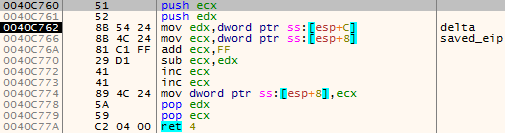
\includegraphics[width=350pt]{obf_func.png}
  \caption{Fonction utilisée pour exécuter une instruction \textit{jmp} de
    manière détournée.}
  \label{fig:func}
\end{figure}

Il y a 11 fonctions comme celle-ci, contenant le même code et qui sont utilisées
à tour de rôle.\\
Dans la figure ci-dessous, la fonction \textit{sage.404924} est une de ces
fonctions.\\

\begin{figure}[H]
  \center
  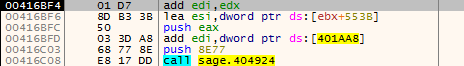
\includegraphics[width=350pt]{obf_usage.png}
  \caption{Utilisation de la fonction pour rendre le flot d'exécution plus
    difficile à suivre.}
  \label{fig:usage}
\end{figure}
\ \\
L'essentiel du code du ransomware est stocké chiffré en mémoire. Le chargement
du code se fait en 2 parties.\\
D'abord, un \textit{stub} (qui est stocké à l'adresse 0x004210BA, chiffré
par des combinaisons de \textit{xor} et de \textit{add})
\footnote{Dans le domaine du packing, un stub est un morceau de code minimal
dont le rôle est de charger une partie plus importante du code qui est chifrée
ou compressée} est déchiffré, copié dans un espace mémoire alloué dynamiquement
puis exécuté.\\
Ce stub se charge ensuite de re-allouer les pages à partir de
l'adresse 0x00400000 (adresse à laquelle est chargée l'image de l'exécutable
en mémoire), supprimant toutes traces des headers et de la section \textit{text}
originale. Il déchiffre ensuite le véritable code du ransomware (qui est
stocké à l'adresse 0x0042166A, chiffré à l'aide de RC4), puis passe
l'exécution au code fraichement déchiffré. Après avoir fait un dump de la partie
packée, on retrouve la véritable liste des fonctions importées ainsi que le
point d'entrée du programme original qui est à l'adresse 0x00406020.\\

\begin{figure}[H]
  \center
  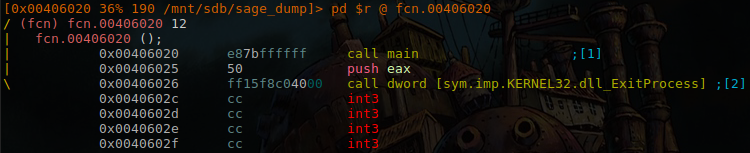
\includegraphics[width=350pt]{oep.png}
  \caption{Point d'entrée du code original, après déchiffrement}
  \label{fig:oep}
\end{figure}

\ \\
Sage n'intègre pas de véritables fonctionnalités d'anti-debug mais tente
simplement de gêner les utilisateurs de débugueurs en simulant un fork au
début de son exécution.
Pour se faire plus discret, Sage tente également de dissimuler sa présence
en faisant une copie de lui-même dans le dossier
\textbf{\%appdata\%\textbackslash Roaming\textbackslash}. Cette copie est nommée
aléatoirement (nom composé de 8 caractères alphanumériques) et c'est elle qui
s'exécute à chaque démarrage de session utilisateur pour assurer la persistance.

\subsection{Main}
Grâce au dump du code original du ransomware, une analyse statique plus
pousée est possible. Bonne nouvelle, la fonction principale est plutôt courte et
sa structure est simple :
\begin{figure}[H]
  \center
  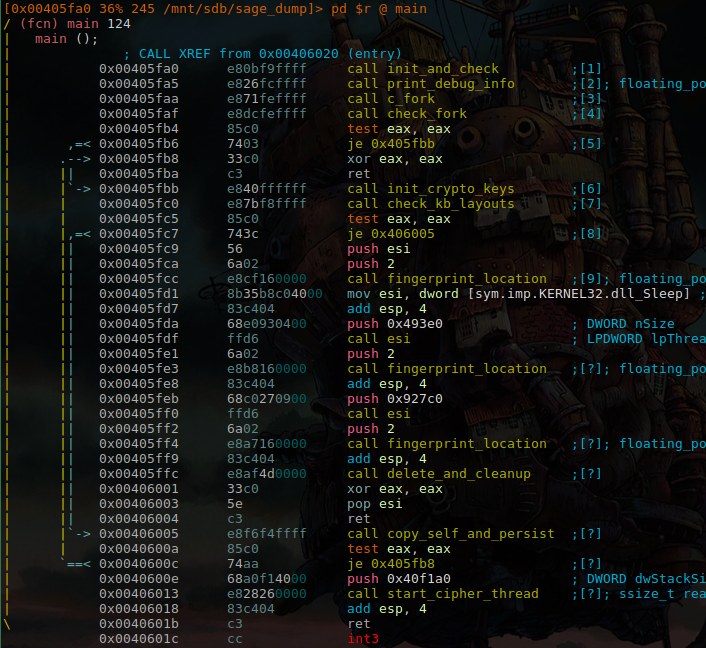
\includegraphics[width=350pt]{main.png}
  \caption{Code assembleur de la fonction principale après déchiffrement}
  \label{fig:main}
\end{figure}

Ce qui donne, en pseudo-code :
\begin{lstlisting}
int main()
{
  init_and_chek();
  print_debug_info();
  c_fork(arg);
  if (check_fork())
    return 0;
  init_crypto_keys();
  if (check_kb_layouts())
  {
    fingerprint_location(2);
    Sleep(0x493E0u);
    fingerprint_location(2);
    Sleep(0x927C0u);
    fingerprint_location(2);
    delete_and_cleanup();
    result = 0;
  }
  else
  {
    if (!copy_self_and_persist())
      return 0;
    result = start_cipher_thread(&encryption_key);
  }
  return result;
}
\end{lstlisting}

\paragraph{Vérification de la langue}
Sage estime la nationalité de la victime, d'après la liste des layouts clavier
utilisés sur la machine, qu'il obtient grâce à la fonction
\textit{GetKeyboardLayoutList}.

\begin{lstlisting}
bool check_kb_layouts()
{
  localeCount = GetKeyboardLayoutList(10, (HKL *)&List);
  if (localeCount <= 0)
    return false;
  i = 0;
  if (localeCount <= 0)
    return false;
  while (true)
  {
    next = (int)(&List)[i] & 0x3FF;
    if (next == 0x23 || next == 0x3F || next == 0x19 || next == 0x22 ||
         next == 0x43 || next == 0x85)
      break;
    if (++i >= localeCount)
      return false;
  }
  return true;
}
\end{lstlisting}
Ces codes correspondent aux layouts clavier suivants :
\begin{itemize}
\item Biélorusse
\item Kazakh
\item Russe
\item Ukrainien
\item Ouzbek
\item Sakha
\end{itemize}
\ \\
Si un de ces layouts clavier est utilisé sur la machine victime, alors Sage
s'arrête avant de chiffrer quoi que ce soit.

\paragraph{Estimation de la localisation}
Si c'est possible (c'est-à-dire, si des bornes Wi-Fi sont détectées), Sage tente
également de localiser plus précisement la machine sur laquelle il s'exécute en
utilisant l'
\href{https://developers.google.com/maps/documentation/geolocation/intro}
{API de géolocalisation Google}.\\
Cette API permet d'estimer la localisation d'une borne Wi-Fi à l'aide de son
adresse MAC et de son SSID.

\paragraph{Persistance}
En ce qui concerne la persistance (l'exécution de lui-même au démarrage),
Sage fait usage des tâches planifiées de Windows. Après s'être copié dans
le dossier \textbf{AppData\textbackslash Roaming\textbackslash}, Sage ajoute une tâche dans la liste
de manière à relancer l'exécution de son binaire à chaque nouvelle connexion
d'un utilisateur sur la machine. Ceci permet de s'assurer que la machine
reste inutilisable après l'infection et ce jusqu'à ce que la rançon
soit payée.\\

\begin{figure}[H]
  \center
  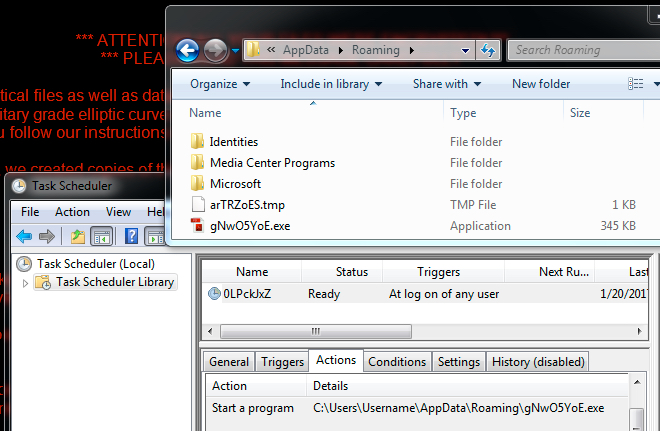
\includegraphics[width=350pt]{persis_task.jpg}
  \caption{Binaire de sage et tâche planifiée utilisée pour maintenir
    l'exécution au démarrage.}
  \label{fig:task}
\end{figure}


\paragraph{Information de debug \& fichier canary}
Certains restes de fonctionnalités de debug sont trouvables dans l'exécutable.
Notamment, la gestion d'un paramètre "d", qui permet d'afficher une information
concernant la configuration du ransomware.

\begin{figure}[H]
  \center
  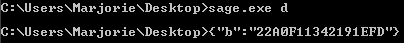
\includegraphics[width=350pt]{debug.jpg}
  \caption{Résultat renvoyé par Sage en lui passant l'argument "d"}
  \label{fig:task}
\end{figure}

Également, vérification de la présence d'un fichier qui permet d'éviter le
lancement du ransomware, certainement utile pour éviter tout lancement
accidentel durant le développement du ransomware :
\begin{lstlisting}
if (CreateFileW(L"C:\\Temp\\lol.txt", 0x80000000, FILE_SHARE_READ, NULL,
     OPEN_EXISTING, 0, NULL) == INVALID_HANDLE_VALUE)
{
	// Chiffrement des fichiers
}
\end{lstlisting}

\paragraph{Communication C\&C}
Sage tente de communiquer à un serveur C\&C durant son exécution. Il essaye
d'abord d'obtenir une adresse IP pour le nom de domaine
\textbf{mbfce24rgn65bx3g.rzunt3u2.com}, et si il n'y parvient pas, envoie
un paquet chiffré à des milliers d'adresses IP différentes en utilisant le
protocole UDP. Le choix du protocole UDP est probablement dû au fait que le
protocole UDP permet d'envoyer un paquet à un serveur sans établir de connexion
ou même attendre de réponse du serveur avec lequel on communique. Cela
permet à Sage de garder la véritable IP du serveur C\&C cachée parmis les
milliers d'IP auxquelles sont envoyés ces paquets.\\

Voici une partie du traffic réseau produit par Sage :
\begin{figure}[H] 
  \center
  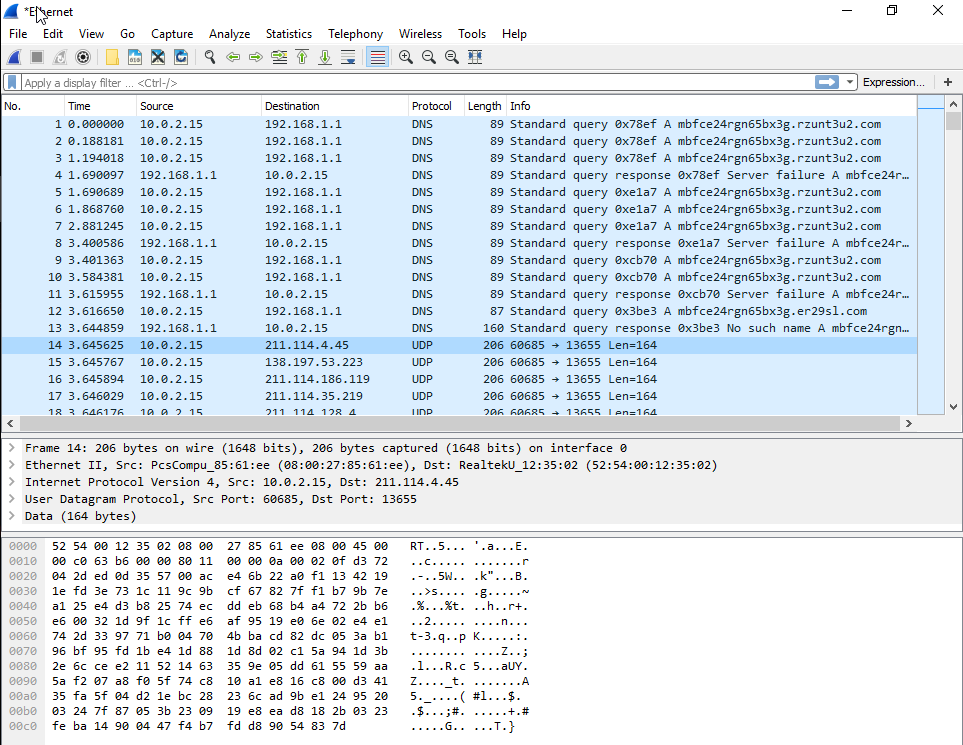
\includegraphics[width=350pt]{packet_log.png}
  \caption{Packets envoyés par Sage lors de son exécution.}
  \label{fig:packets}
\end{figure}

\subsection{Extensions ciblées}
Pour éviter de rendre le système d'exploitation inutilisable en chiffrant des
fichiers critiques, les ransomwares se contentent de chiffrer uniquement les
fichiers dont les noms contiennent les extensions les plus couramment utilisées
pour les fichiers de données utilisateur.\\
En ce qui concerne Sage, cette liste est la suivante :
\begin{lstlisting}
.dat .mx0 .cd .pdb .xqx .old .cnt .rtp .qss .qst .fx0 .fx1 .ipg .ert .pic .img
.cur .fxr .slk .m4u .mpe .mov .wmv .mpg .vob .mpeg .3g2 .m4v .avi .mp4 .flv
.mkv .3gp .asf .m3u .m3u8 .wav .mp3 .m4a .m .rm .flac .mp2 .mpa .aac .wma .djv
.pdf .djvu .jpeg .jpg .bmp .png .jp2 .lz .rz .zipx .gz .bz2 .s7z .tar .7z .tgz
.rar .zip .arc .paq .bak .set .back .std .vmx .vmdk .vdi .qcow .ini .accd .db
.sqli .sdf .mdf .myd .frm .odb .myi .dbf .indb .mdb .ibd .sql .cgn .dcr .fpx
.pcx .rif .tga .wpg .wi .wmf .tif .xcf .tiff .xpm .nef .orf .ra .bay .pcd .dng
.ptx .r3d .raf .rw2 .rwl .kdc .yuv .sr2 .srf .dip .x3f .mef .raw .log .odg .uop
.potx .potm .pptx .rss .pptm .aaf .xla .sxd .pot .eps .as3 .pns .wpd .wps .msg
.pps .xlam .xll .ost .sti .sxi .otp .odp .wks .vcf .xltx .xltm .xlsx .xlsm
.xlsb .cntk .xlw .xlt .xlm .xlc .dif .sxc .vsd .ots .prn .ods .hwp .dotm .dotx
.docm .docx .dot .cal .shw .sldm .txt .csv .mac .met .wk3 .wk4 .uot .rtf .sldx
.xls .ppt .stw .sxw .dtd .eml .ott .odt .doc .odm .ppsm .xlr .odc .xlk .ppsx
.obi .ppam .text .docb .wb2 .mda .wk1 .sxm .otg .oab .cmd .bat .h .asx .lua .pl
.as .hpp .clas .js .fla .py .rb .jsp .cs .c .jar .java .asp .vb .vbs .asm .pas
.cpp .xml .php .plb .asc .lay6 .pp4 .pp5 .ppf .pat .sct .ms11 .lay .iff .ldf
.tbk .swf .brd .css .dxf .dds .efx .sch .dch .ses .mml .fon .gif .psd .html
.ico .ipe .dwg .jng .cdr .aep .aepx .123 .prel .prpr .aet .fim .pfb .ppj .indd
.mhtm .cmx .cpt .csl .indl .dsf .ds4 .drw .indt .pdd .per .lcd .pct .prf .pst
.inx .plt .idml .pmd .psp .ttf .3dm .ai .3ds .ps .cpx .str .cgm .clk .cdx .xhtm
.cdt .fmv .aes .gem .max .svg .mid .iif .nd .2017 .tt20 .qsm .2015 .2014 .2013
.aif .qbw .qbb .qbm .ptb .qbi .qbr .2012 .des .v30 .qbo .stc .lgb .qwc .qbp
.qba .tlg .qbx .qby .1pa .ach .qpd .gdb .tax .qif .t14 .qdf .ofx .qfx .t13 .ebc
.ebq .2016 .tax2 .mye .myox .ets .tt14 .epb .500 .txf .t15 .t11 .gpc .qtx .itf
.tt13 .t10 .qsd .iban .ofc .bc9 .mny .13t .qxf .amj .m14 ._vc .tbp .qbk .aci
.npc .qbmb .sba .cfp .nv2 .tfx .n43 .let .tt12 .210 .dac .slp .qb20 .saj .zdb
.tt15 .ssg .t09 .epa .qch .pd6 .rdy .sic .ta1 .lmr .pr5 .op .sdy .brw .vnd .esv
.kd3 .vmb .qph .t08 .qel .m12 .pvc .q43 .etq .u12 .hsr .ati .t00 .mmw .bd2 .ac2
.qpb .tt11 .zix .ec8 .nv .lid .qmtf .hif .lld .quic .mbsb .nl2 .qml .wac .cf8
.vbpf .m10 .qix .t04 .qpg .quo .ptdb .gto .pr0 .vdf .q01 .fcr .gnc .ldc .t05
.t06 .tom .tt10 .qb1 .t01 .rpf .t02 .tax1 .1pe .skg .pls .t03 .xaa .dgc .mnp
.qdt .mn8 .ptk .t07 .chg .#vc .qfi .acc .m11 .kb7 .q09 .esk .09i .cpw .sbf .mql
.dxi .kmo .md .u11 .oet .ta8 .efs .h12 .mne .ebd .fef .qpi .mn5 .exp .m16 .09t
.00c .qmt .cfdi .u10 .s12 .qme .int? .cf9 .ta5 .u08 .mmb .qnx .q07 .tb2 .say
.ab4 .pma .defx .tkr .q06 .tpl .ta2 .qob .m15 .fca .eqb .q00 .mn4 .lhr .t99
.mn9 .qem .scd .mwi .mrq .q98 .i2b .mn6 .q08 .kmy .bk2 .stm .mn1 .bc8 .pfd .bgt
.hts .tax0 .cb .resx .mn7 .08i .mn3 .ch .meta .07i .rcs .dtl .ta9 .mem .seam
.btif .11t .efsl .$ac .emp .imp .fxw .sbc .bpw .mlb .10t .fa1 .saf .trm .fa2
.pr2 .xeq .sbd .fcpa .ta6 .tdr .acm .lin .dsb .vyp .emd .pr1 .mn2 .bpf .mws
.h11 .pr3 .gsb .mlc .nni .cus .ldr .ta4 .inv .omf .reb .qdfx .pg .coa .rec .rda
.ffd .ml2 .ddd .ess .qbmd .afm .d07 .vyr .acr .dtau .ml9 .bd3 .pcif .cat .h10
.ent .fyc .p08 .jsd .zka .hbk .mone .pr4 .qw5 .cdf .gfi .cht .por .qbz .ens
.3pe .pxa .intu .trn .3me .07g .jsda .2011 .fcpr .qwmo .t12 .pfx .p7b .der .nap
.p12 .p7c .crt .csr .pem .gpg .key
\end{lstlisting}

\subsection{Chiffrement}
Sage se démarque des autres ransomwares en ce qui concerne le chiffrement
puisqu'il fait usage de cryptographie sur les courbes elliptiques ainsi que
de l'algorithme ChaCha pour chiffrer les fichiers de l'utilisateur, ce qui
n'est pas commun.\\
ChaCha est un algortihme de chiffrement à flot dérivé de Salsa20; Sage l'utilise
pour chiffrer le contenu des fichiers.\\
Chaque fichier cible est renommé et chiffré avec une clé ChaCha
choisie aléatoirement, et cette clé est ensuite stockée à la fin du fichier
chiffré. Cette clé n'est évidemment pas stockée tel quel dans le fichier, ce
sont en fait deux parties qui permettent, si on possède une valeur secrète, de
retrouver la clé utilisée pour chiffrer le fichier, qui sont stockées.\\
Il est important de noter que Sage prend soin de supprimer les sauvegardes
de fichiers faites avec \textit{Shadow Copy} avant de commencer le chiffrement.
\ \\
Les calculs sont faits sur la courbe elliptique \textit{Curve25519} (d'équation
$y^2 = x^3 + 486662*x^2 + x$, sur $\mathbb{F}_p = GF(2^{255} - 19)$), qui est
une courbe populaire pour plusieurs raisons (sécurité, rapidité des calculs,
propriétés liées à la génération d'éléments aléatoires) et qui est conçue pour
être utilisée par le protocole ECDH (Elliptic Curve Diffie-Hellman).\\
Dans la suite, on notera $\mathbb{F}_p = GF(2^{255} - 19)$ et $G$ le point de
la courbe $Curve25519$ admettant $x = 9$. Enfin, le ransomware a connaissance de
$Q_s = k_s * G$, la partie publique de l'extorqueur utilisée lors de la création
du secret partagé.\\
Le chiffrement d'un fichier se déroule comme ceci :
\begin{itemize}
\item On génère $k_c \in \mathbb{F}_p$ aléatoirement
\item On calcule le point $Q_c = k_c * G$
\item On calcule le secret partagé $S = k_c * Q_s = (k_c * k_s) * G$
\item On dérive du secret partagé, un entier $sh \in \mathbb{F}_p$
\item On calcule le point $P = sh * G$
\item On génère $n \in \mathbb{F}_p$ aléatoirement
\item On calcule les points $chacha\_key = n * P = (n * sh) * G$ et
  $chacha\_pub = n * G$
\item On chiffre le fichier en utilisant ChaCha avec une clé dérivée de
  $chacha\_key$ 
\item On ajoute les valeurs de $Q_c$ et $chacha\_pub$ à la fin du fichier
\end{itemize}
\ \\

Ce qui produit, en pratique, un fichier de la forme :
\begin{figure}[H]
  \center
  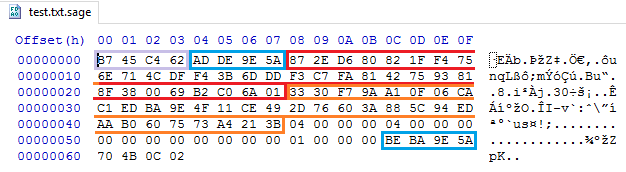
\includegraphics[width=350pt]{dump_file.png}
  \caption{Contenu d'un fichier après avoir été chiffré par Sage.}
  \label{fig:file}
\end{figure}
\ \\
Légende :
\begin{itemize}
\item Mauve : Contenu chiffré du fichier original
\item Rouge : $Q_c$
\item Orange : $chacha\_pub$
\item Bleu : Valeurs constantes
\end{itemize}

Petite note sur le déchiffrement; il est nécéssaire de connaître la valeur
de $k_s$ pour pouvoir déchiffrer les fichiers. Cette valeur n'est stockée
nulle part dans le binaire et on peut donc supposer que seul l'auteur du
ransomware la possède, évidemment. Étant donné qu'il n'est donc pas possible,
en pratique, de calculer $k_s$ en un temps raisonnable, le seul moyen de
déchiffrer les fichiers est donc, soit de payer, soit d'attendre que la clé
privée fuite ou soit retrouvée sur des serveurs saisis par la police (comme ce
fut le cas pour le ransomware ICEPOL).\\
Le déchiffrement d'un fichier se déroule comme ceci :
\begin{itemize}
\item On récupère les valeurs $Q_c$ et $chacha\_pub$
\item On calcule le secret partagé $S = k_s * Q_c = (k_s * k_c) * G$
\item On dérive du secret partagé, l'entier $sh \in \mathbb{F}_p$
\item On calcule le point $chacha\_key = sh * chacha\_pub = (sh * n) * G$
\item On déchiffre le fichier en utilisant ChaCha avec la clé dérivée
  de $chacha\_key$
\end{itemize}


\chapter*{Conclusion}

Les études du botnet Ganiw et du ransomware SageCrypt ont permis d'effleurer la
diversité des malwares présents aujourd'hui. Ces deux malwares sont très
différents dans leurs structures et dans les protections mises en place.\\
Ganiw est codé de manière très modulaire et ses protections contre
le reverse-engineering sont assez faible. C'est un malware facilement analysable
mais qui pourra être retrouvé sous de nombreuses formes,
avec des modules d'attaques supplémentaires.
À l'inverse, SageCrypt est bien plus protégé, avec la présence
d'un packer par exemple, mais son code et sa structure sont plus ou moins connus,
car dérivés d'un autre ransomware, CryLocker.\\

À la suite de cette étude, il est facile de remarquer que du temps peut être
économisé en automatisant certaines parties de l'étude, qui plus est si
l'élément a inspecté ou que ses mécanismes d'infection et de propagation
sont déjà, en partie connus, et si de nombreux éléments sont à étudier.
Parmi les outils existants sont disponibles les sandboxs
\textit{Limon}\footnote{\url{https://github.com/monnappa22/Limon}} et
\textit{Cuckoo}\footnote{\url{https://github.com/cuckoosandbox/cuckoo}},
très utiles pour fournir rapidement de nombreuses informations sur l'élément
analysé et de manière sécurisé, sans compromettre son environnement de travail.\\

Mais ceci ne permet pas de classifier les malwares et nécessite encore
une grande partie de travail manuel. Pour cela, il faudrait pouvoir les
discriminer en fonction de leur comportement, de leurs appels
à diverses librairies, \ldots Ceci pourrait être fait en se basant sur
le graphe du flot d'exécution (CFG: Control Flow Graph), mais devra être fiable
et les analyses de malware ne pourront se passer d'actions humaines pour
identifier de nouvelles formes de menaces.


% -- For Biblio --
%\nocite{*}
%\bibliographystyle{plain}
%\bibliography{biblio}

\end{document}
